\documentclass{article}
\usepackage{graphicx} % Required for inserting images
\usepackage{wrapfig}

\title{PS6 Zilles}
\author{Andrew Zilles}
\date{March 2024}

\begin{document}

\maketitle

\section{In your .tex file, tell me about the steps you took to clean and transform the data.
}
So I wanted to get some sort of live baseball data. Originally I just wanted to get the live score of games, but Supertramp wrote a song about taking the long way home and I wanted to relate to that. The problem I was facing is that most live data APIs required a subscription/setup and a credit card on file to use their data. (Apparently people really like to use their APIs for sports betting and they want their fair share.) So my friend Reddit suggested using the ESPN API and I just decided to piggyback off that and scrape their data. Their site is nice because each game is assigned a unique ID and then you can see play by play data by putting /playbyplay/ in the url. I pulled the tables from the game I wanted to track and found that I need to merge the table with the team names and the table with the actual scores. That was a fun learning experience but didn't feel like enough. I then got a wild idea that I could write a script that would pull their schedule, check if they had a game that day, if they did it would then pull up the /playbyplay/ site and update every minute or so in order to show the live score.

I got to work pulling the schedule from ESPN. I walked in the mud for quite a while and kept thinking that I could just pull the schedule from another site or even just the baseballr package. I decided to keep going though because it would be nice to have all the data coming from one source. In my R script I tried to document my steps to do that. Is this the easiest way? Frick no. Am I really just reinventing the wheel? Yes. But I made that wheel and I'm proud of it and this is probably the first coding "challenge" I've had to solve this semester so it was fun to do.

Steps:
\begin{enumerate}
    \item ESPN likes to break their schedule up into three sections (sping training, regular season, and post season) with the second section being split into two halves. The nice thing is that this is only done with a change at the end of each site with a 1/2/3. I learned that my code will still work with the 2024 postseason even though that's not a reality yet because it just redirects it to another schedule. So the postseason code has been written but hashed out.
    \item I then wanted to include additional info on the tables about the games. The good news is that this data is all contained in the ESPN hyperlink. The bad news is that hyperlink isn't part of the table, so I added it. I then did some playing with the table to extract the unique game ID assigned by ESPN, the home team, and the away team.
    \item Because I was using a simple strsplit function on the last part of the hyperlink to get team nicknames it had some issues. When the team nickname was two words (Blue Jays, Red Sox, White Sox) it would only show one word. So there was basic find and replace to correct these instances.
    \item After all the data for each schedule section was aligned, I merged them on top of each other to create one schedule to rule them all and show their entire season.
    \item Then to add some more data so that I could make a cool map plot I added the stadium address of the home team where the game would be played. This is not 100 percent accurate because I didn't include the actual stadiums where they played their spring training games (so my data could show them playing baseball in an open sky field in Minnesota in late February - whoops.) 
    \item I also included this when I was making the visualizations but I really could have included it up here. I add a column of what the team's main color is (thanks Copilot for automatically generating that code for me!) so that I can make the charts look all fancy(ish).
\end{enumerate}

I would have liked to go a little farther with this and actually create the script that runs and checks for games on a daily basis but I've already more time than I have on this. Part of my process was to extract the unique game ID and put it in the schedule table. So theoretically it could be easy to write something that checks the schedule every day and flag when a today's date matches a date on the schedule. When it has been flagged it will pull the unique game ID and concatenate a url with the ID and the /playbyplay/ text. And then I could have another function that scrapes the url created site and outputs the live score. The schedule table also has the game start time so I'm thinking that could also be used as the "start time" for when the /playbyplay/ table gets created and initiates a refresh of the table every so often until the game is over. I'm not sure if ESPN will like that, but I'll probably never get around to making it so the concern is resolved.

\section{Include in your .tex file an explanation of what the images are communicating. How
are they helpful for understanding your data set?
}
This begins our artistic tour where the budding artist displays his best interpretations of life, humanity, and the futility of man.

We begin with Figure 1, this was created at a time in the artist's life when he was pursing a PhD and liked learning about coding but had demands to complete other works. You can see by his use of color that he really wanted to invoke the spirit of each team represented here. Graphically depicted, we can see how often the Houston Astros play in each stadium away from home (excluding post season appearances and the spring training technicality spoken to above.) One is left to wonder why he chose to keep such a long data label for each of the stadiums? Is this a sign of his inexperience or an artistic choice? Did he choose to leave it like this because he ran out of time or because he thought it would really catch the viewer's attention and pull their eyes upwards towards the colored bars? The world may never know.
\begin{figure}
    \centering
    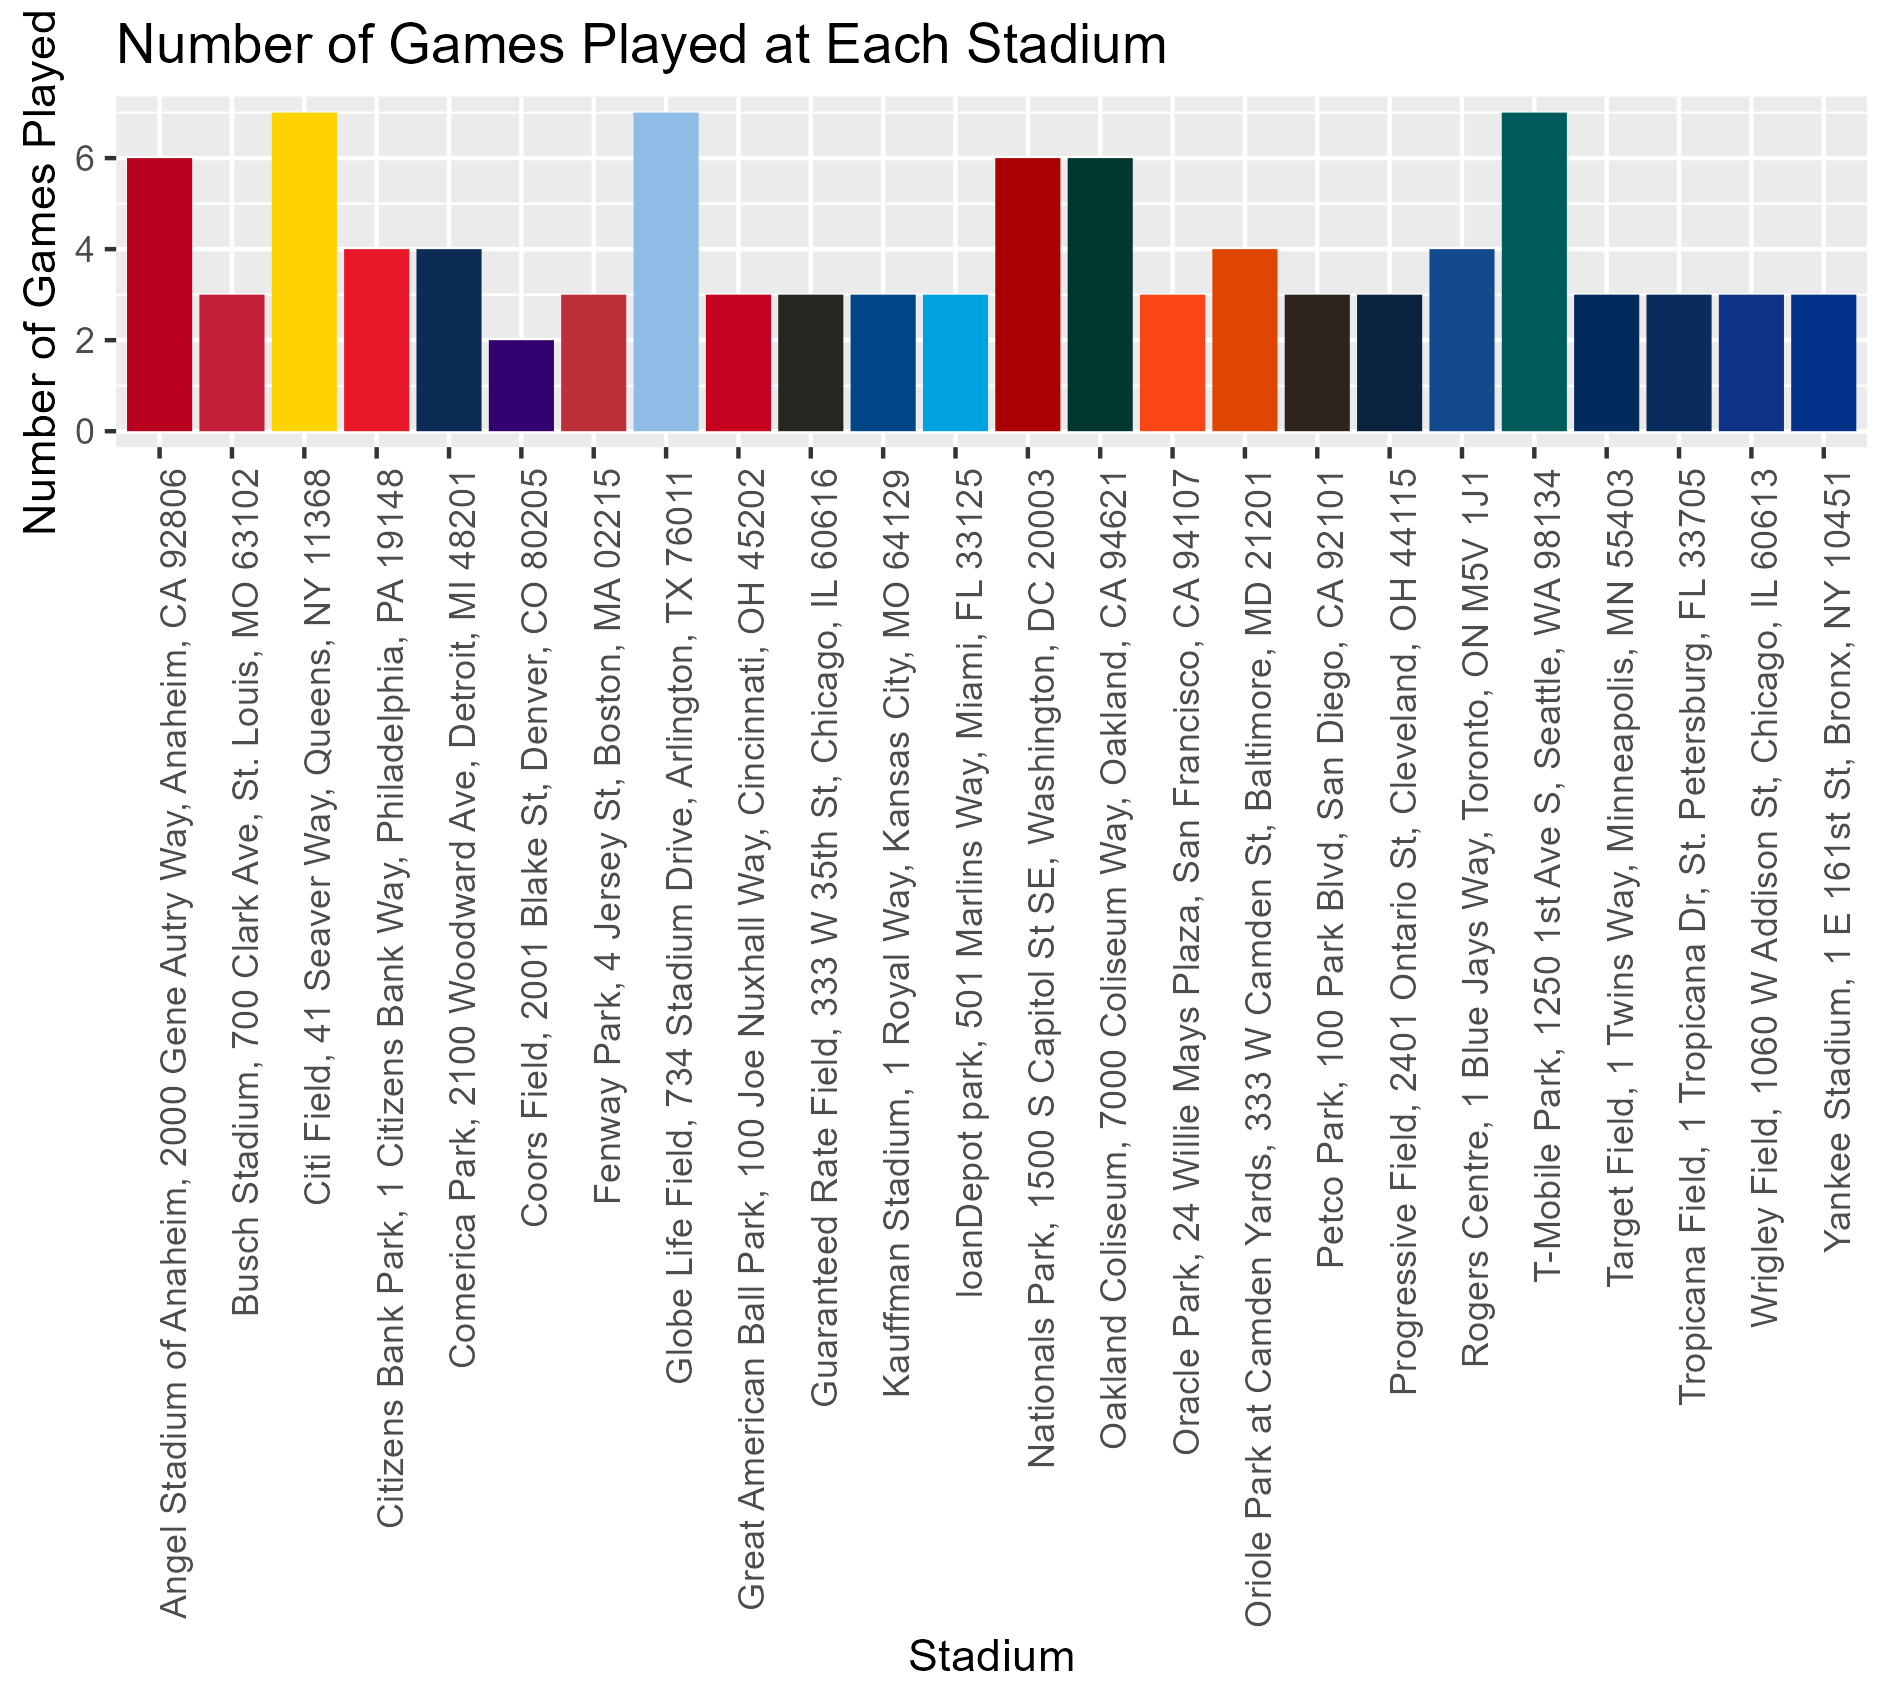
\includegraphics[width=0.5\linewidth]{PS6a_Zilles.png}
    \caption{1890 x 1703, pixels on screen (or ink on paper, depending on what meuseum you view this at)}
    \label{fig:Frequency of Stadiums}
\end{figure}

Next, we move on to Figure 2. This work came after the artist had experimented with Figure 1 but had apprenticed with other masters. You can start to see the influence of his closest mentor, the honorable master ChatGPT. Opting to display the bars horizontally and ordered based on magnitude is a break from his prior work. This graph shows the number of games played against each opponent (home or away). We begin to see a much more polished work in this era of the artist's life.
\begin{figure}
    \centering
    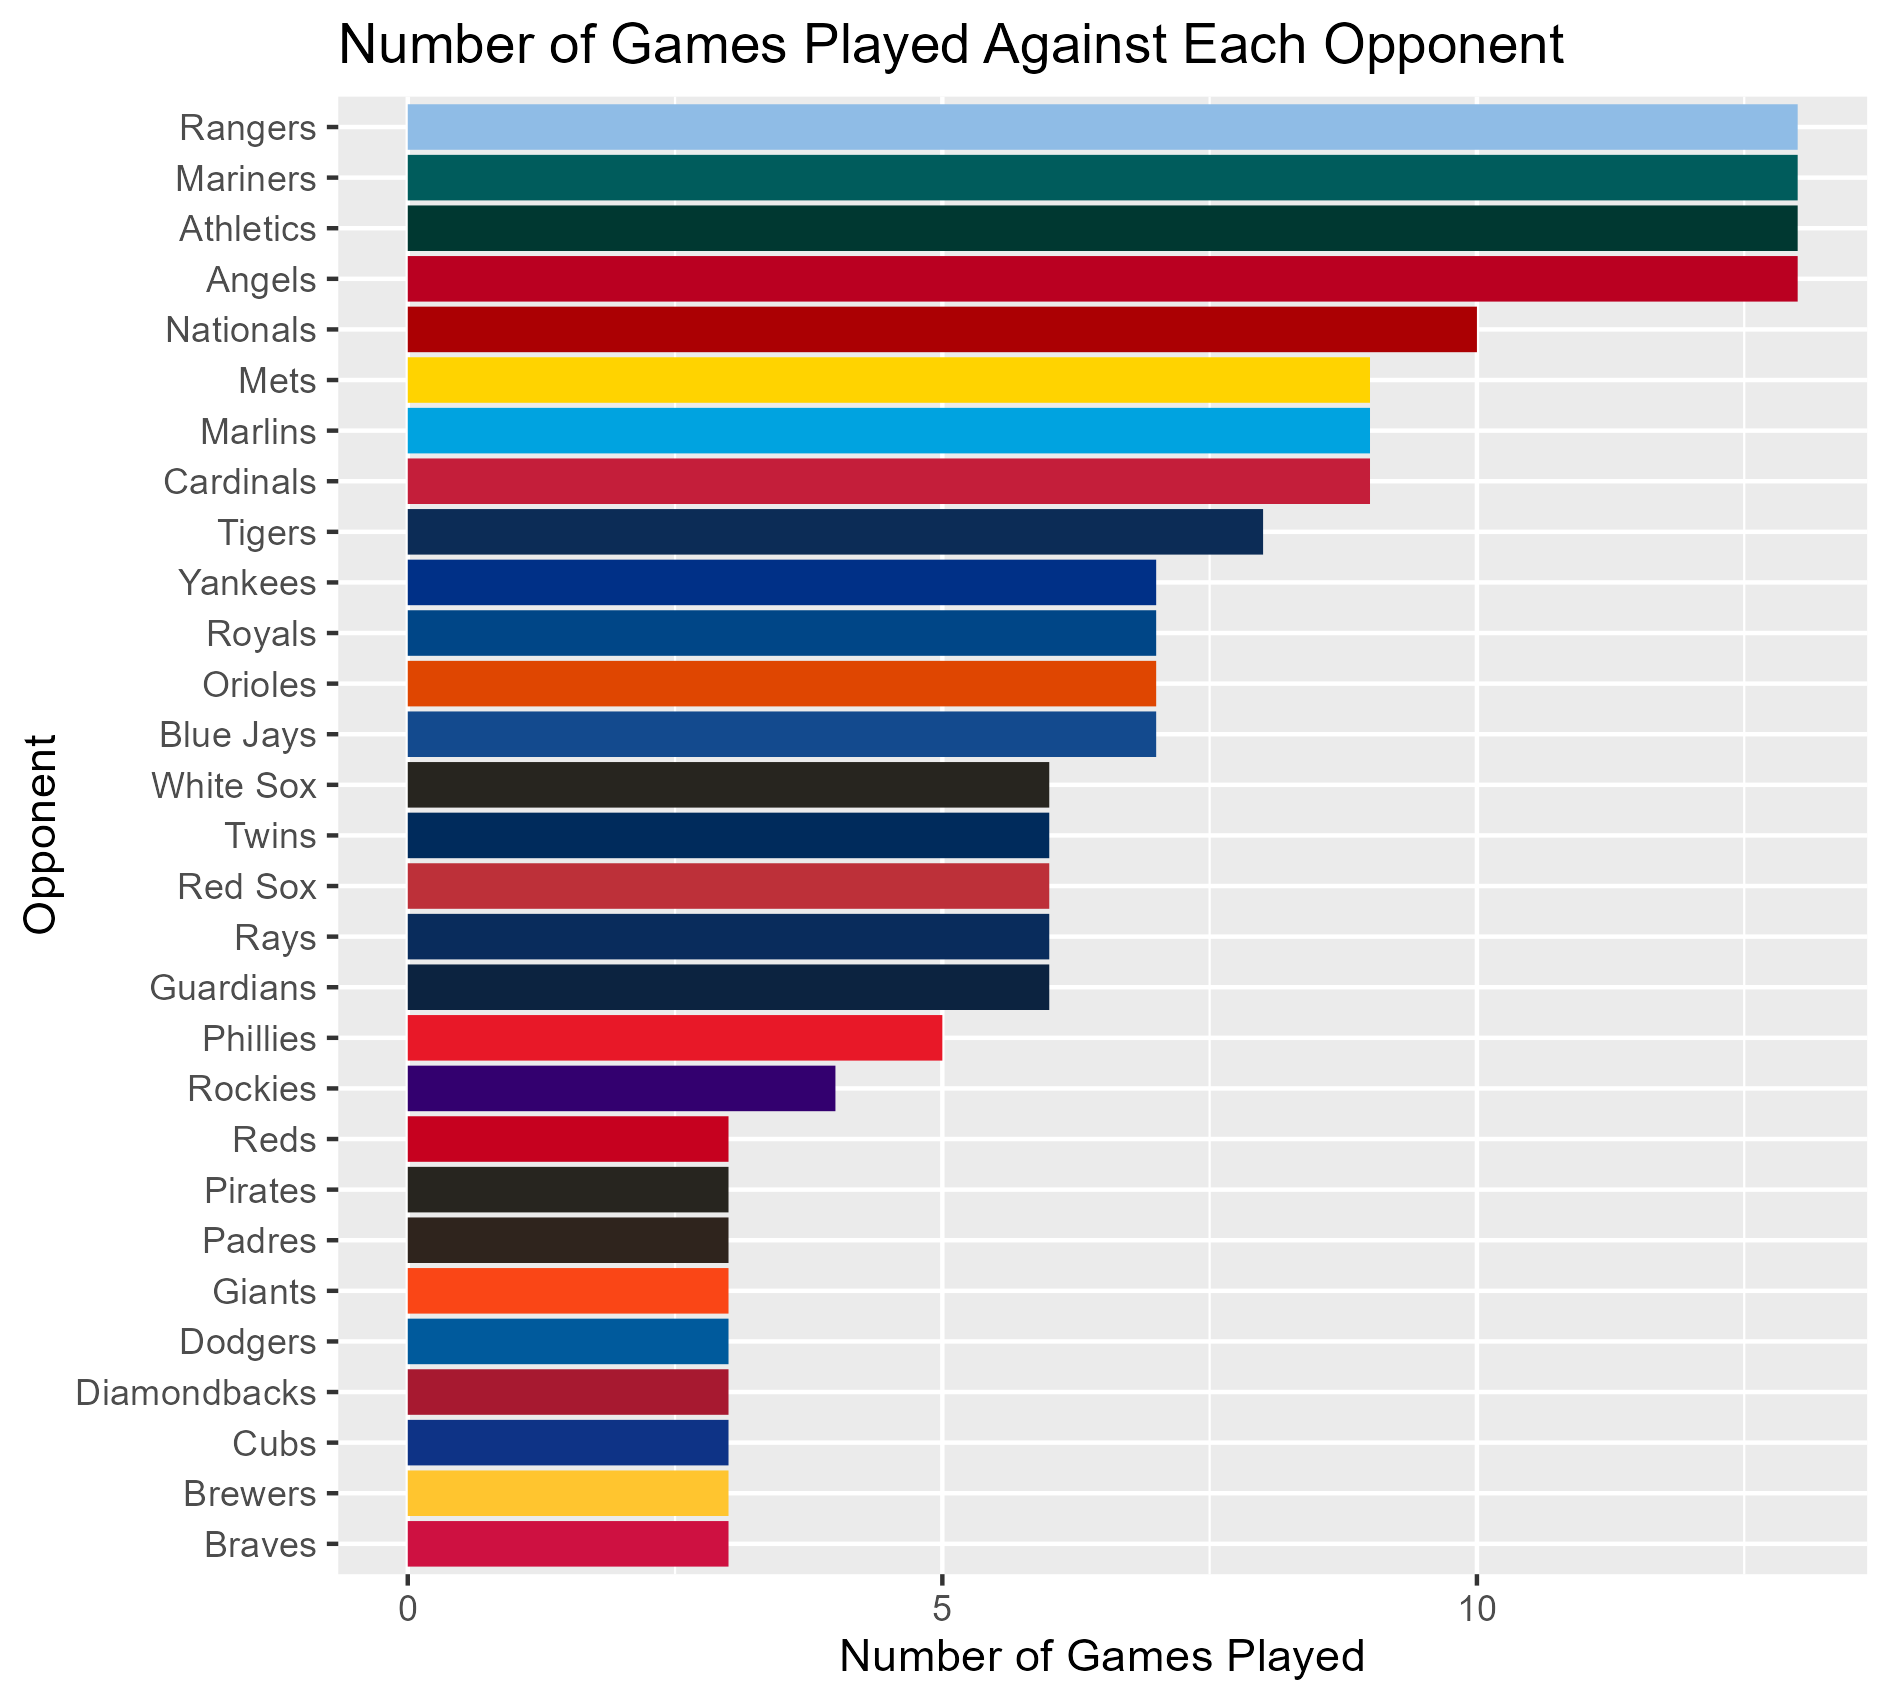
\includegraphics[width=0.5\linewidth]{PS6b_Zilles.png}
    \caption{1890 x 1703, pixels on screen}
    \label{fig:enter-label}
\end{figure}

We conclude with this piece in the artist's last days. We can see much more advanced techniques in use, requiring a departure from the standard mediums. Critics quickly pointed out how useless the heat map of this graph is and that it could be much better served with dropped pins or an integration calculating the distance between the away team's stadium relative to the Astro's home stadium. The artist never addressed these critics directly and instead pointed out that they didn't understand art. One wonders if he was ahead of his time or just too experimental. Later in his life he would admit that his graph was his least favorite to produce and that he felt rushed to complete it and get it out of his shop. Common at the time, LSD could have played a major part in this work. The artist denies such claims.
\begin{figure}
    \centering
    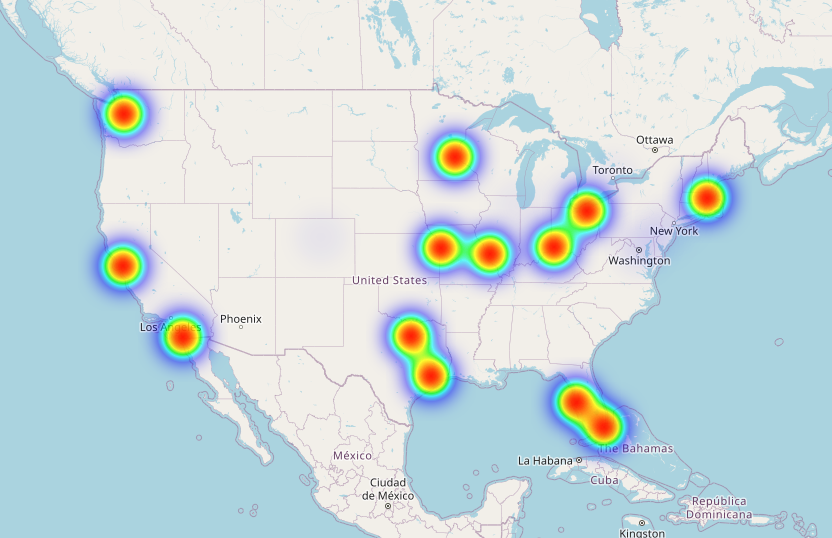
\includegraphics[width=0.5\linewidth]{PS6c_Zilles.png}
    \caption{832 x 538, pixels on screen}
    \label{fig:enter-label}
\end{figure}

These three works clearly demonstrate the early beginnings, peak, and slow descent of the artist throughout the lifespan of this assignment. Will this artist have a Renaissance?
\end{document}
